% In preamble:
% \usepackage{pgfplots}
% \pgfplotsset{compat=1.18}

\begin{figure}[htbp]
\centering
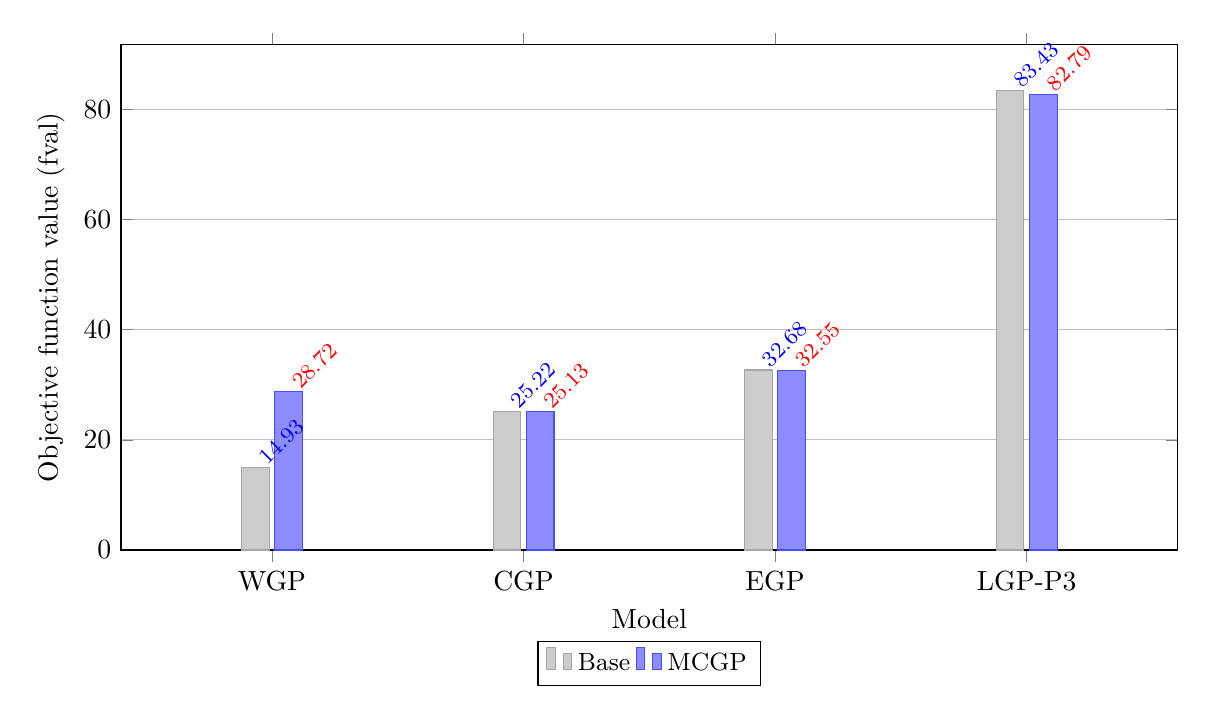
\begin{tikzpicture}
\begin{axis}[
  ybar,
  bar width=10pt,
  width=15cm,
  height=8cm,
  ymin=0,
  ylabel={Objective function value (fval)},
  xlabel={Model},
  symbolic x coords={WGP,CGP,EGP,LGP-P3},
  xtick=data,
  enlarge x limits=0.2,
  ymajorgrids,
  legend style={at={(0.5,-0.18)},anchor=north,legend columns=2,font=\small},
nodes near coords,
nodes near coords style={rotate=45, anchor=west, font=\footnotesize},
  every node near coord/.append style={font=\footnotesize}
]

% Base models
\addplot+[fill=gray!40, draw=gray!70]
  coordinates {(WGP,14.9277) (CGP,25.2174) (EGP,32.6816) (LGP-P3,83.4264)};
\addlegendentry{Base}

% MCGP
\addplot+[fill=blue!45, draw=blue!70]
  coordinates {(WGP,28.7245) (CGP,25.1304) (EGP,32.5462) (LGP-P3,82.7889)};
\addlegendentry{MCGP}

\end{axis}
\end{tikzpicture}
\caption{Comparison of \textit{fval} for Base vs.\ MCGP variants across models.}
\label{fig:fval_base_vs_mcgp}
\end{figure}
